%!TEX root = /Users/louis/Documents/PhD/Deliverables/Thesis/thesis.tex

% TODO - I probably need to introduce model-metamodel co-evolution here, to make the method and structure sections more understandable. It might be possible to include an example of evolution in MDE in this chapter, and to identify types of evolution including model-metamodel co-evolution.

\chapter{Introduction}
\label{Introduction}
Today's software developers build distributed and interoperating systems with sophisticated graphical interfaces rather than the insular, monolithic, and command-line driven mainframe applications built by their predecessors. The National Programme for IT\footnote{\url{http://www.connectingforhealth.nhs.uk/about/benefits/statement0607.pdf}} seeks to modernise the United Kingdom's National Health Service (NHS) by replacing paper for computerised systems in managing the nation's patient records. 

Some of the software demanded by users and developers today is so complicated that its construction is not possible, even using state-of-the-art software engineering techniques \cite{selic03pragmatics}. However, demand does not appear to exceed capability in all areas of computer science.

%\cite{pool97society} observes that a similar situation occurred when steam and electrical power were introduced during the Industrial Revolution. 

Hardware development, for example, seems to advance more quickly than software development. Each year, faster personal computers with larger disk drives become available, while operating systems, office software and development environments seem to improve more gradually. \cite{brooks86nosilverbullet} suggests that radical advances in software development occur only by raising the level of abstraction at which software is specified.

%  

% \cite{brooks86nosilverbullet} observes that engineering increasingly complicated systems with traditional development approaches presents many challenges, including:
% 
% \begin{enumerate}
%  \item \textit{Increasing size of development teams}: large teams may experience communication difficulties, detracting from productivity.
%  \item \textit{Difficulties providing system overviews}: incomplete system knowledge can impede maintenance activities.
%  \item \textit{Poor understandability}: new developers suffer a complex learning curve.
%  \item \textit{Resistance to change}: development reacts slowly when requirements change, new underlying technologies are to be adopted, and unintended behaviour must be corrected.
% \end{enumerate}
% 
% 
% 
% Improvements to development processes have also facilitated greater abstraction. For example, developers are increasingly employing models of systems to aid design and implementation. During the 1990s, methods that prescribed modelling to aid software development were popular. A common modelling language, the Unified Modelling Language (UML) \cite{uml212}, was standardised by combining the modelling languages from three methods \cite{}. By communicating designs and abstracting away from unimportant details, software engineers are using models to address the first three of Brooks's challenges. However, modelling is effective only when the models are an accurate representation of the computer system.

% During a system's lifecycle, design documents are often neglected and become out-of-date. Without a well-defined connection to the system's implementation, models are effectively design documents that might be neglected and can become inaccurate representations of the system \cite{frankel02mda,kleppe03mda}. For models to be used as effective means of communication and education, they must be accurate and, therefore, must be maintained and updated in response to change. Maintaining two unconnected representations of a system (models and implementation) obviously detracts from the productivity of the development team. Instead, an approach to software development that integrates modelling and coding can be used to address this productivity problem, as well as the first three of Brooks's challenges.


%!TEX root = /Users/louis/Documents/PhD/Deliverables/Thesis/thesis.tex

\section{Model-Driven Engineering}
Historically, raising the level of abstraction of software development has led to increased productivity. For example, assembly language provides mnemonics for machine code, allowing developers to disregard superfluous detail (such as the binary representation of instructions). Object-orientation and functional programming permit further abstraction over assembler, enabling developers to express solutions in a manner that is more representative of their problem domain.

Model-Driven Engineering (MDE) is a contemporary approach to software engineering that seeks to abstract away from technological details (such as programming languages and off-the-shelf software components) and towards the problem domain of the system (for example: accounting, managing patient records, or searching the Internet). To this end, MDE prescribes, throughout the software engineering process, the use of models to capture the relevant details of the problem domain. Software development is driven by manipulating (transforming, validating, merging, comparing, etc.) the models to automatically generate working code.

MDE reportedly provides many benefits over traditional approaches to software engineering. \cite{watson08mdahistory} presents results from two unpublished case studies, and suggests that MDE can lead to increased productivity by reducing the amount of time to develop a system, and by reducing the number of defects discovered throughout development. \cite{kleppe03mda} discusses the ways in which MDE can be used to increase the productivity of software development and the maintainability and portability of software systems.

Notwithstanding its benefits, MDE introduces additional challenges for software development. \cite{kolovos08scalability} reports scalability issues with contemporary MDE, noting that large models are commonplace in many software engineering projects and that contemporary MDE environments cannot be used to manipulate large models. \cite{Mens07} demonstrate that MDE introduces new challenges for managing change throughout the lifetime of a system. This thesis focuses on the latter challenge, which is part of a branch of computer science termed \emph{software evolution}.

\section{Software Evolution}
Software changes over time. During the lifetime of a software system, unintended behaviour must be corrected and new requirements satisfied. Because modern software systems are rarely isolated from other systems, changes are also made to facilitate interoperability with new systems \cite{sjoberg93quantifying}. 

% \cite{lehman80understanding,lehman78programs,lehman69programming} identify several laws of software evolution for \textit{evolutionary-type systems} (\textit{E-type systems}) -- systems that solve problems or implement software in the real world. E-type systems differ from \textit{specification-type systems} (\textit{S-type systems}) where the ``sole criterion of acceptability is correctness in the mathematical sense'' \cite{lehman85program}.
% 
% The law of \textit{continuing change} states that ``E-type systems must be continually adapted else they become progressively less satisfactory'' \cite{lehman78programs}. Later, Lehman et al. \cite{lehman96laws} introduce another complementary law, the law of \textit{declining quality}: ``The quality of E-type systems will appear to be declining unless they are rigorously maintained and adapted to operational environment change''. Both laws indicate that the evolution of E-type systems during their effective lifetime is inevitable.

\emph{Software evolution} is an area of computer science that focuses on the way in which a software system changes over time in response to external pressures (such as changing requirements, or the discovery of unintended behaviour). The terms software evolution and software maintenance are used interchangeably in the software engineering literature. In this thesis, \emph{evolution} is preferred to \emph{maintenance}, because the latter can imply deterioration caused by repeated use, and most software systems do not deteriorate in this manner \cite{ramil00cost}. Other than sharing some terminology, software evolution is not related to evolutionary algorithms, a branch of computer science that encompasses genetic programming and genetic algorithms. 

In the past, studies have suggested that software evolution can account for as much as 90\% of a development budget \cite{erlikh00leveraging,moad90maintaining}, and there is no reason to believe that the situation is different today. Although \cite[ch. 21]{sommerville06software} describes such figures as uncertain, precise figures are not required to demonstrate that the effects of evolution can inhibit the productivity of software development.

For example, suppose that we are developing a software system using a combination of hand-written code and off-the-shelf components. Part way through development, one of the components changes to support a new requirement. When using the new version of the component, we must first determine whether our system exhibits any unintended behaviour, identify the cause of the unintended behaviour, and change the system accordingly. The resources allocated to correcting any unintended behaviour are not being used to develop features for the users of our system.

Primarily, software evolution research seeks to reduce the cost of making changes to a system. Analysis of the effects of evolution facilitates informed decisions about how best to manage evolution. For example, analysis of our system might indicate that using a new version of a component will introduce three defects, but simplify the implementation of two features. Studying the way in which systems evolve lead to improvements in software development tools and processes that reduce the effects of evolution. For example, contemporary software development environments recognise compilation as a common activity during software evolution, and often perform automatic and incremental compilation of source code in the background. Future changes to a system might be anticipated by identifying the ways in which the system has previously evolved. For example, understanding the ways in which our system has been affected by using a new version of a component might highlight ways in which our system can be better protected against changes to its dependencies.

% TODO - might need to relate the above points to productivity, understandability and portability

% By understanding the mistakes made in the engineering of existing software systems, similar mistakes may be avoided in the future. Experts and analysts can devise best practices that guide developers away from problematic practices. For this reason, Kerievsky notes that ``studying the evolution of great software designs will be more valuable than studying the great designs themselves'' \cite{kerievsky04refactoring}.


%!TEX root = /Users/louis/Documents/PhD/Deliverables/Thesis/thesis.tex

\section{Software Evolution Challenges in MDE}
%!TEX root = /Users/louis/Documents/PhD/Deliverables/Thesis/thesis.tex

\section{Research Hypothesis}
The research presented in this thesis explores the following hypothesis:

\begin{quote}
\emph{In existing MDE projects, evolution is typically managed in an ad-hoc manner with little regard for re-use. Dedicated structures and processes for identifying and managing evolutionary change can be designed by analysing evolution in existing MDE projects. Furthermore, supporting those dedicated structures and processes in contemporary MDE environments is beneficial in terms of increased \textbf{productivity}, \textbf{understandability}, and \textbf{portability}.}
\end{quote}

Some of the terms used in the research hypothesis are ambiguous, and require further definition. Specifically, the terms productivity, understandability and portability are defined as follows:

\paragraph{Productivity} is a measure of the amount of work required to complete a development activity. For example, the productivity of data entry might be increased by using an Optical Character Recognition (OCR) system rather than a typist. In this scenario, the extent to which productivity might be increased is affected by at least the following: the accuracy and capabilities of the OCR system, the speed and accuracy of the typist, and the legibility and consistency of the data. In general, productivity is affected by many factors.

% Productivity
%  HUTN + MMIS for user-driven co-evolution
%  A choice of user-driven vs developer-driven co-evolution
%  Dedicated migration lang rather than M2M lang for model migration 

\paragraph{Understandability} is a measure of the ease with which the purpose, motivation and workings of a system can be identified from the representation of that system. For example, the function of a circuit is arguably easier to understand when examining a schematic of the circuit rather than a Printed Circuit Board (PCB) that implements the circuit. For example, components are often arranged to save space on a PCB, while components might be arranged to ease understanding of the system on a schematic. Clearly, understandability is somewhat subjective. Due to differences in knowledge and experience, a representation that is easy to understand for one person may be difficult for another. 

% Understandability
%  Flock for expressing model migration
%  Use of design patterns / refactorign terminology to describe metamodel evolution
%  HUTN rather than XMI for representating non-conformant models

\paragraph{Portability} is a measure of the extent to which a system can be changed to interoperate with other systems. For example, a system implemented directly in machine code can be used with only one family of machines, while an equivalent system implemented in a high-level language (and compiled to machine code) can be used with different families of machine. Hence, the latter is more portable than the former.

% Portability:
%  Migrating between modelling technologies
%  Higher-order migration (migrating between transformation [and other model management?] languages)

\subsection{Thesis Objectives}
The objectives of the thesis are to:

\begin{enumerate}
	\item Identify and analyse evolutionary change in existing MDE projects.
	\item Investigate the extent to which existing structures and processes for identifying and managing evolutionary change can be used in MDE. 
	\item Develop new structures and processes for identifying and managing evolutionary change in the context of MDE, and integrate those structures and processes with a contemporary MDE development environment.
	\item Evaluate and assess new and existing structures and processes for identifying and managing evolutionary change, particularly with respect to productivity, understandability and portability.
\end{enumerate}
%!TEX root = /Users/louis/Documents/PhD/Deliverables/Thesis/thesis.tex

\section{Research Method}
\label{sec:research_method}
To explore the hypothesis outlined above, the thesis research was conducted using the method described in this section and summarised in Figure~\ref{fig:research_method}. The green boxes represent the three \emph{phases} of research, which are described below. The white boxes represent inputs and outputs to those phases.

%This section will discuss the way in which the research was conducted, including a description of the evaluation strategy.

% TODO - Need to highlight that lower level research objectives are identified in analysis and implementation chapters. This can probably also be explained in the method section 

\begin{figure}[htbp]
  \begin{center}
    \leavevmode
    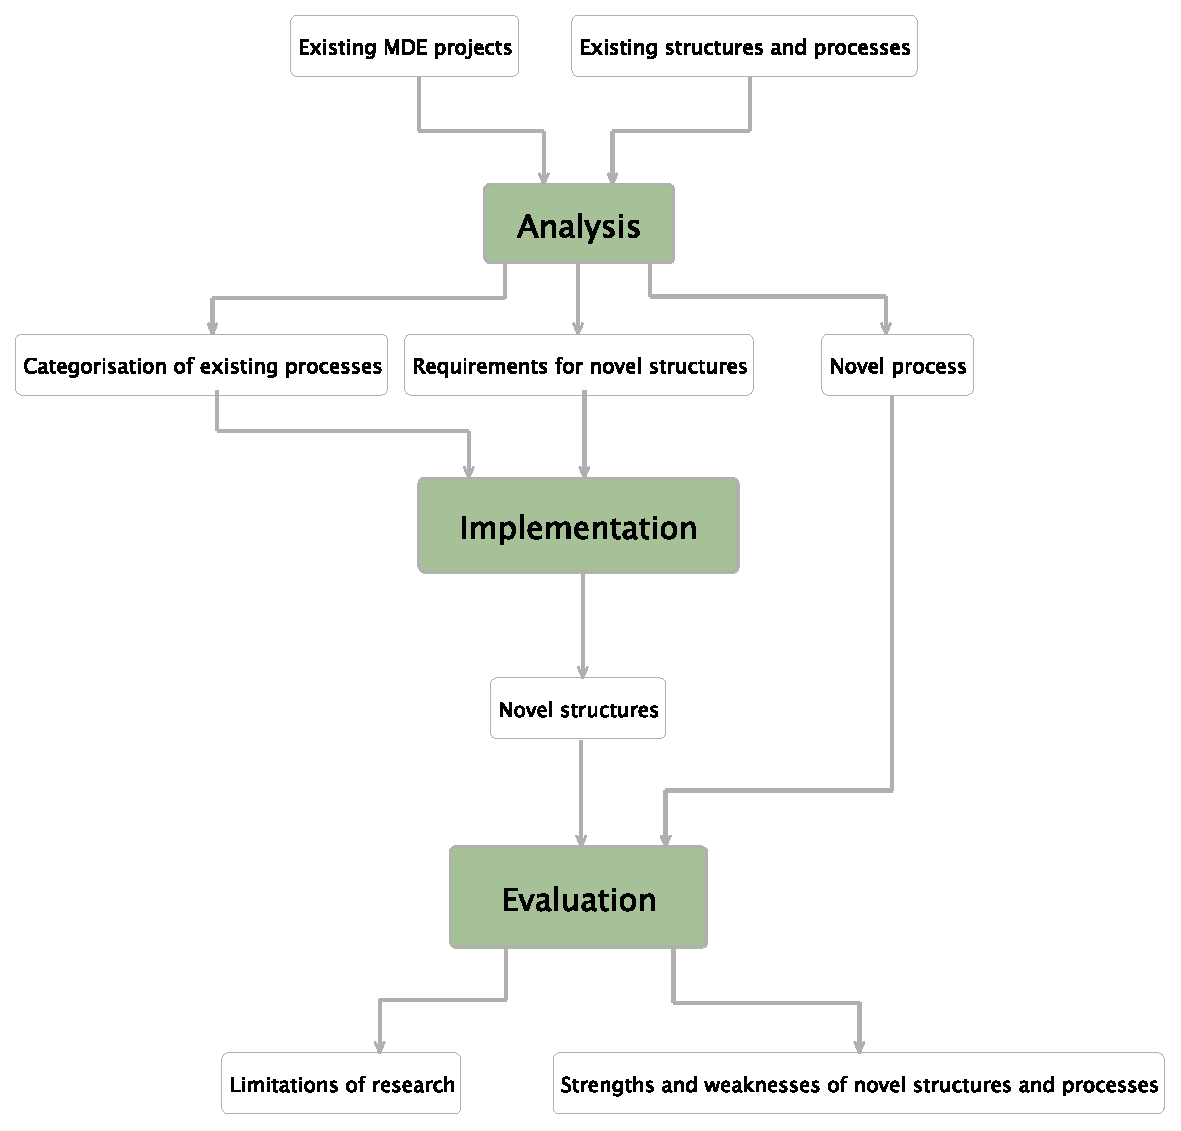
\includegraphics[width=12cm]{1.Introduction/images/method.pdf}
  \end{center}
  \caption{Overview of the research method.}
  \label{fig:research_method}
\end{figure}


Firstly, the \emph{analysis} phase involved studying the evolution of MDE development artefacts in existing projects. The results of the analysis phase were used to determine a category of evolution that lacked support in contemporary MDE development environments, \emph{model-metamodel co-evolution} or, simply \emph{co-evolution}. Co-evolution examples from existing MDE projects were used to categorise existing processes for managing co-evolution, and to formulate requirements for new structures and processes for managing co-evolution. The analysis phase also lead to the identification of \emph{user-driven co-evolution}, a process for managing co-evolution that has not previously been recognised in the co-evolution literature.

The \emph{implementation} phase involved proposing, designing and implementing novel structures for managing co-evolution, and integrating the structures with a contemporary MDE environment. The co-evolution examples identified in the analysis phase were used for testing the implementation of the structures.

The \emph{evaluation} phase involved assessing the novel structures for managing co-evolution by comparison to existing structures, and demonstrating the novel process. Evaluation was performed using further examples of co-evolution. To mitigate a possible threat to the validity of the research, the examples used in the evaluation phase were different to those used in the analysis phase. The strengths and weaknesses of the novel and existing structures and processes were synthesised from the comparisons, particularly with respect to the productivity and understandability of software development.

A similar method was used successfully in \cite{dig07thesis} to explore the extent to which component-based applications can be automatically evolved. Initially, \cite{dig06apis} conducted \emph{analysis} to identify and categorise evolution in five existing component-based applications, with the hypothesis that many of the changes could be classified as behaviour-preserving. By using examples from the survey, \cite{dig06detection} were able to \emph{implement} an algorithm for automatically detecting behaviour-preserving changes. The algorithm was then used to implement tools for (1) migrating code in a distributed and collaborative software development environment \cite{dig06automatic}, and (2) analysing the history of component-based applications \cite{dig07cms}. The latter facilitated better understanding of program evolution, and refinement of the detection algorithm. Finally, \cite{dig07thesis} \emph{evaluated} the tools and detection algorithm by application to three further component-based applications.
%!TEX root = /Users/louis/Documents/PhD/Deliverables/Thesis/thesis.tex

\section{Research Results}
\label{sec:research_results}

This thesis proposes novel structures and processes for managing model-metamodel co-evolution. Prototypical reference implementations of the proposed structures have been constructed, including \emph{Epsilon HUTN} (a textual modelling notation) and \emph{Epsilon Flock} (a model migration language). The reference implementations have been constructed atop Epsilon \cite{kolovos09thesis}, an extensible platform for specifying MDE languages and tools, and are interoperable with the Eclipse Modelling Framework \cite{steinberg09emf}, arguably the most widely used MDE modelling framework.

Additionally, this thesis identifies a novel process for managing model-metamodel co-evolution and proposes a theoretical categorisation of existing process for managing model-metamodel co-evolution. The novel process, termed \emph{user-driven co-evolution}, is demonstrated by application to a MDE development process for a real-world project.

The research hypothesis has been validated by comparing the prototypes of the proposed structures and processes with existing structures and processes using examples of evolution from real-world MDE projects. Evaluation has been performed using several approaches, including a collaborative comparison of model migration tools carried out with three MDE experts, comparing quantitive measurements of the proposed and existing migration languages, and application of the proposed structures and processes to two examples of evolution, including an example from a widely used modelling language, the Unified Modelling Language (UML) \cite{uml212}. The evaluation also explored areas in which the prototypical implementations of the proposed structures and processes might be usefully improved to be fit for industrial use.


% Productivity
%  HUTN + MMIS for user-driven co-evolution
%  A choice of user-driven vs developer-driven co-evolution
%  Dedicated migration lang rather than M2M lang for model migration

% Understandability
%  Flock for expressing model migration
%  Use of design patterns / refactorign terminology to describe metamodel evolution
%  HUTN rather than XMI for representating non-conformant models

% Might also mention portability:
%  Migrating between modelling technologies
%  Higher-order migration (migrating between transformation [and other model management?] languages)

%!TEX root = /Users/louis/Documents/PhD/Deliverables/Thesis/thesis.tex

\section{Thesis Structure}
Chapter~\ref{Background} gives an overview of MDE by defining terminology; describing associated engineering principles, practices and tools; and reviewing related areas of computer science. Section~\ref{sec:mde_benefits_and_challenges} synthesises some of the benefits of, and challenges for, contemporary MDE.

Chapter~\ref{LiteratureReview} reviews theoretical and practical software evolution research. Areas of research that underpin software evolution are described, including refactoring, design patterns, and traceability. The review then discusses work that approaches particular categories of evolution problem, such as programming language, schema and grammar evolution. Section~\ref{subsec:mde_evo} surveys work that considers evolution in the context of MDE. Section~\ref{sec:literature_review_summary} identifies three types of evolution that occur in MDE projects and highlights challenges for their management.

Chapter~\ref{Analysis} surveys existing MDE projects and categorises the evolution of MDE development artefacts in those projects. From this survey, the context for the thesis research is narrowed, and the remainder of the thesis focuses on one type of evolution occurring in MDE projects, termed \emph{model-metamodel co-evolution} or simply \emph{co-evolution}. Examples of co-evolution are used to identify the strengths and weaknesses of existing structures and processes for managing co-evolution. From this, Section~\ref{subsec:user-driven_co-evolution} identifies a process for managing co-evolution which has not been recognised previously in the literature, Section~\ref{subsec:co-evolution_categorisation} derives a categorisation of existing processes for managing co-evolution, and Section~\ref{sec:requirements_identification} synthesises requirements for novel structures for managing co-evolution.

Chapter~\ref{Implementation} describes novel structures for managing co-evolution, including a metamodel-independent syntax, which is used to identify, report and to facilitate the reconciliation of problems caused by metamodel evolution. The textual modelling notation described in Section~\ref{sec:notation} and the model migration language described in Section~\ref{sec:flock} are used for reconciliation of models in response to metamodel evolution. The latter provides a means for performing reconciliation in a repeatable manner.

Chapter~\ref{Evaluation} assesses the structures and processes proposed in this thesis by comparison to existing structures and processes. To explore the research hypothesis, several different types of comparison were performed, including an experiment in which quantitive measurements were derived, a collaborative comparison of model migration tools with three MDE experts, and application to a large, independent example of evolution taken from a real-world MDE project.

Chapter~\ref{Conclusion} summarises the achievements of the research, and discusses results in the context of the research hypothesis. Limitations of the thesis research and areas of future work are also outlined.

